\documentclass{standalone}
\usepackage{mintikz}

\tikzset{every picture/.style={thick}}

\begin{document}
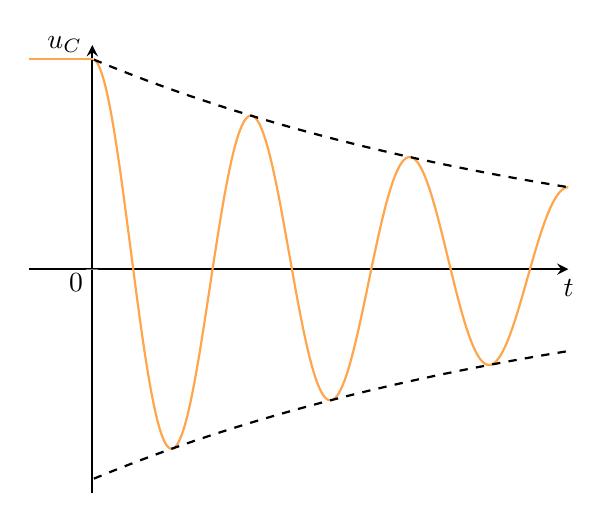
\begin{tikzpicture}[]
	\def\E{3}
	\def\wo{2*pi*0.2}
	\def\w{\wo*sqrt(1-1/(4*\Q^2))}
	\def\Q{10}
	\def\xmax{15}
	\begin{axis}[
			xmin=-2, xmax=\xmax,
			ymin=-3.2, ymax=3.2,
			xlabel=$t$, ylabel=$u_C$,
			axis lines=center,
			xtick=\empty, ytick=\empty,
			extra y ticks={0},
			y tick label style={yshift={(\tick==0)*-.5em},
					xshift={(\tick==0)*.25em}},
			x label style={at={(current axis.right of origin)}, anchor=north, below},
			y label style={at={(current axis.above origin)}, anchor=east, left},
			clip=false]
		\addplot[thick,
			domain=-2:0,
			samples=100,
			orange!70]
		{\E};
		\addplot[thick,
			domain=0.05:\xmax,
			samples=1000,
			orange!70]
		{\E*exp(-\wo*\x/(2*\Q))*(cos(deg(\wo*\x))+1/(sqrt(4*\Q^2-1))*sin(deg(\wo*\x)))};
		\addplot[
			domain=0.05:\xmax,
			smooth, dashed,
			black]
		{\E*exp(-\wo*\x/(2*\Q))};
		\addplot[
			domain=0.05:\xmax,
			smooth, dashed,
			black]
		{-\E*exp(-\wo*\x/(2*\Q))};
	\end{axis}
\end{tikzpicture}
\end{document}
